\documentclass[a4paper]{article}
\usepackage{amssymb}
\usepackage{gensymb}
\usepackage{mhchem}
\usepackage{pgfplots}
\pgfplotsset{width=10cm}
\usepackage{parskip}
\usepackage{multirow}
\usepackage{caption}
\usepackage{graphicx}
\usepackage[
    a4paper,
    left=32mm,
    right=32mm,
    top=40mm,
    bottom=32mm
]{geometry}
\usepackage[T1]{fontenc}
\usepackage[ngerman]{babel}

\graphicspath{ {./} }

% \setlength{\parindent}{0pt}
\renewcommand{\arraystretch}{1.2}

\begin{document}
\section*{Protokoll}
\subsection*{Geräte und Chemikalien}
\begin{itemize}
    \item elektronischer Temperaturmesser
    \item mit Styropor isoliertes Becherglas
    \item $20\textrm{ ml}$ 1-molare Natriumhydroxidlösung
    \item $20\textrm{ ml}$ 1-molare Schwefelsäure
\end{itemize}

\subsection*{Aufbau}
\begin{figure*}[h]
    \centering
    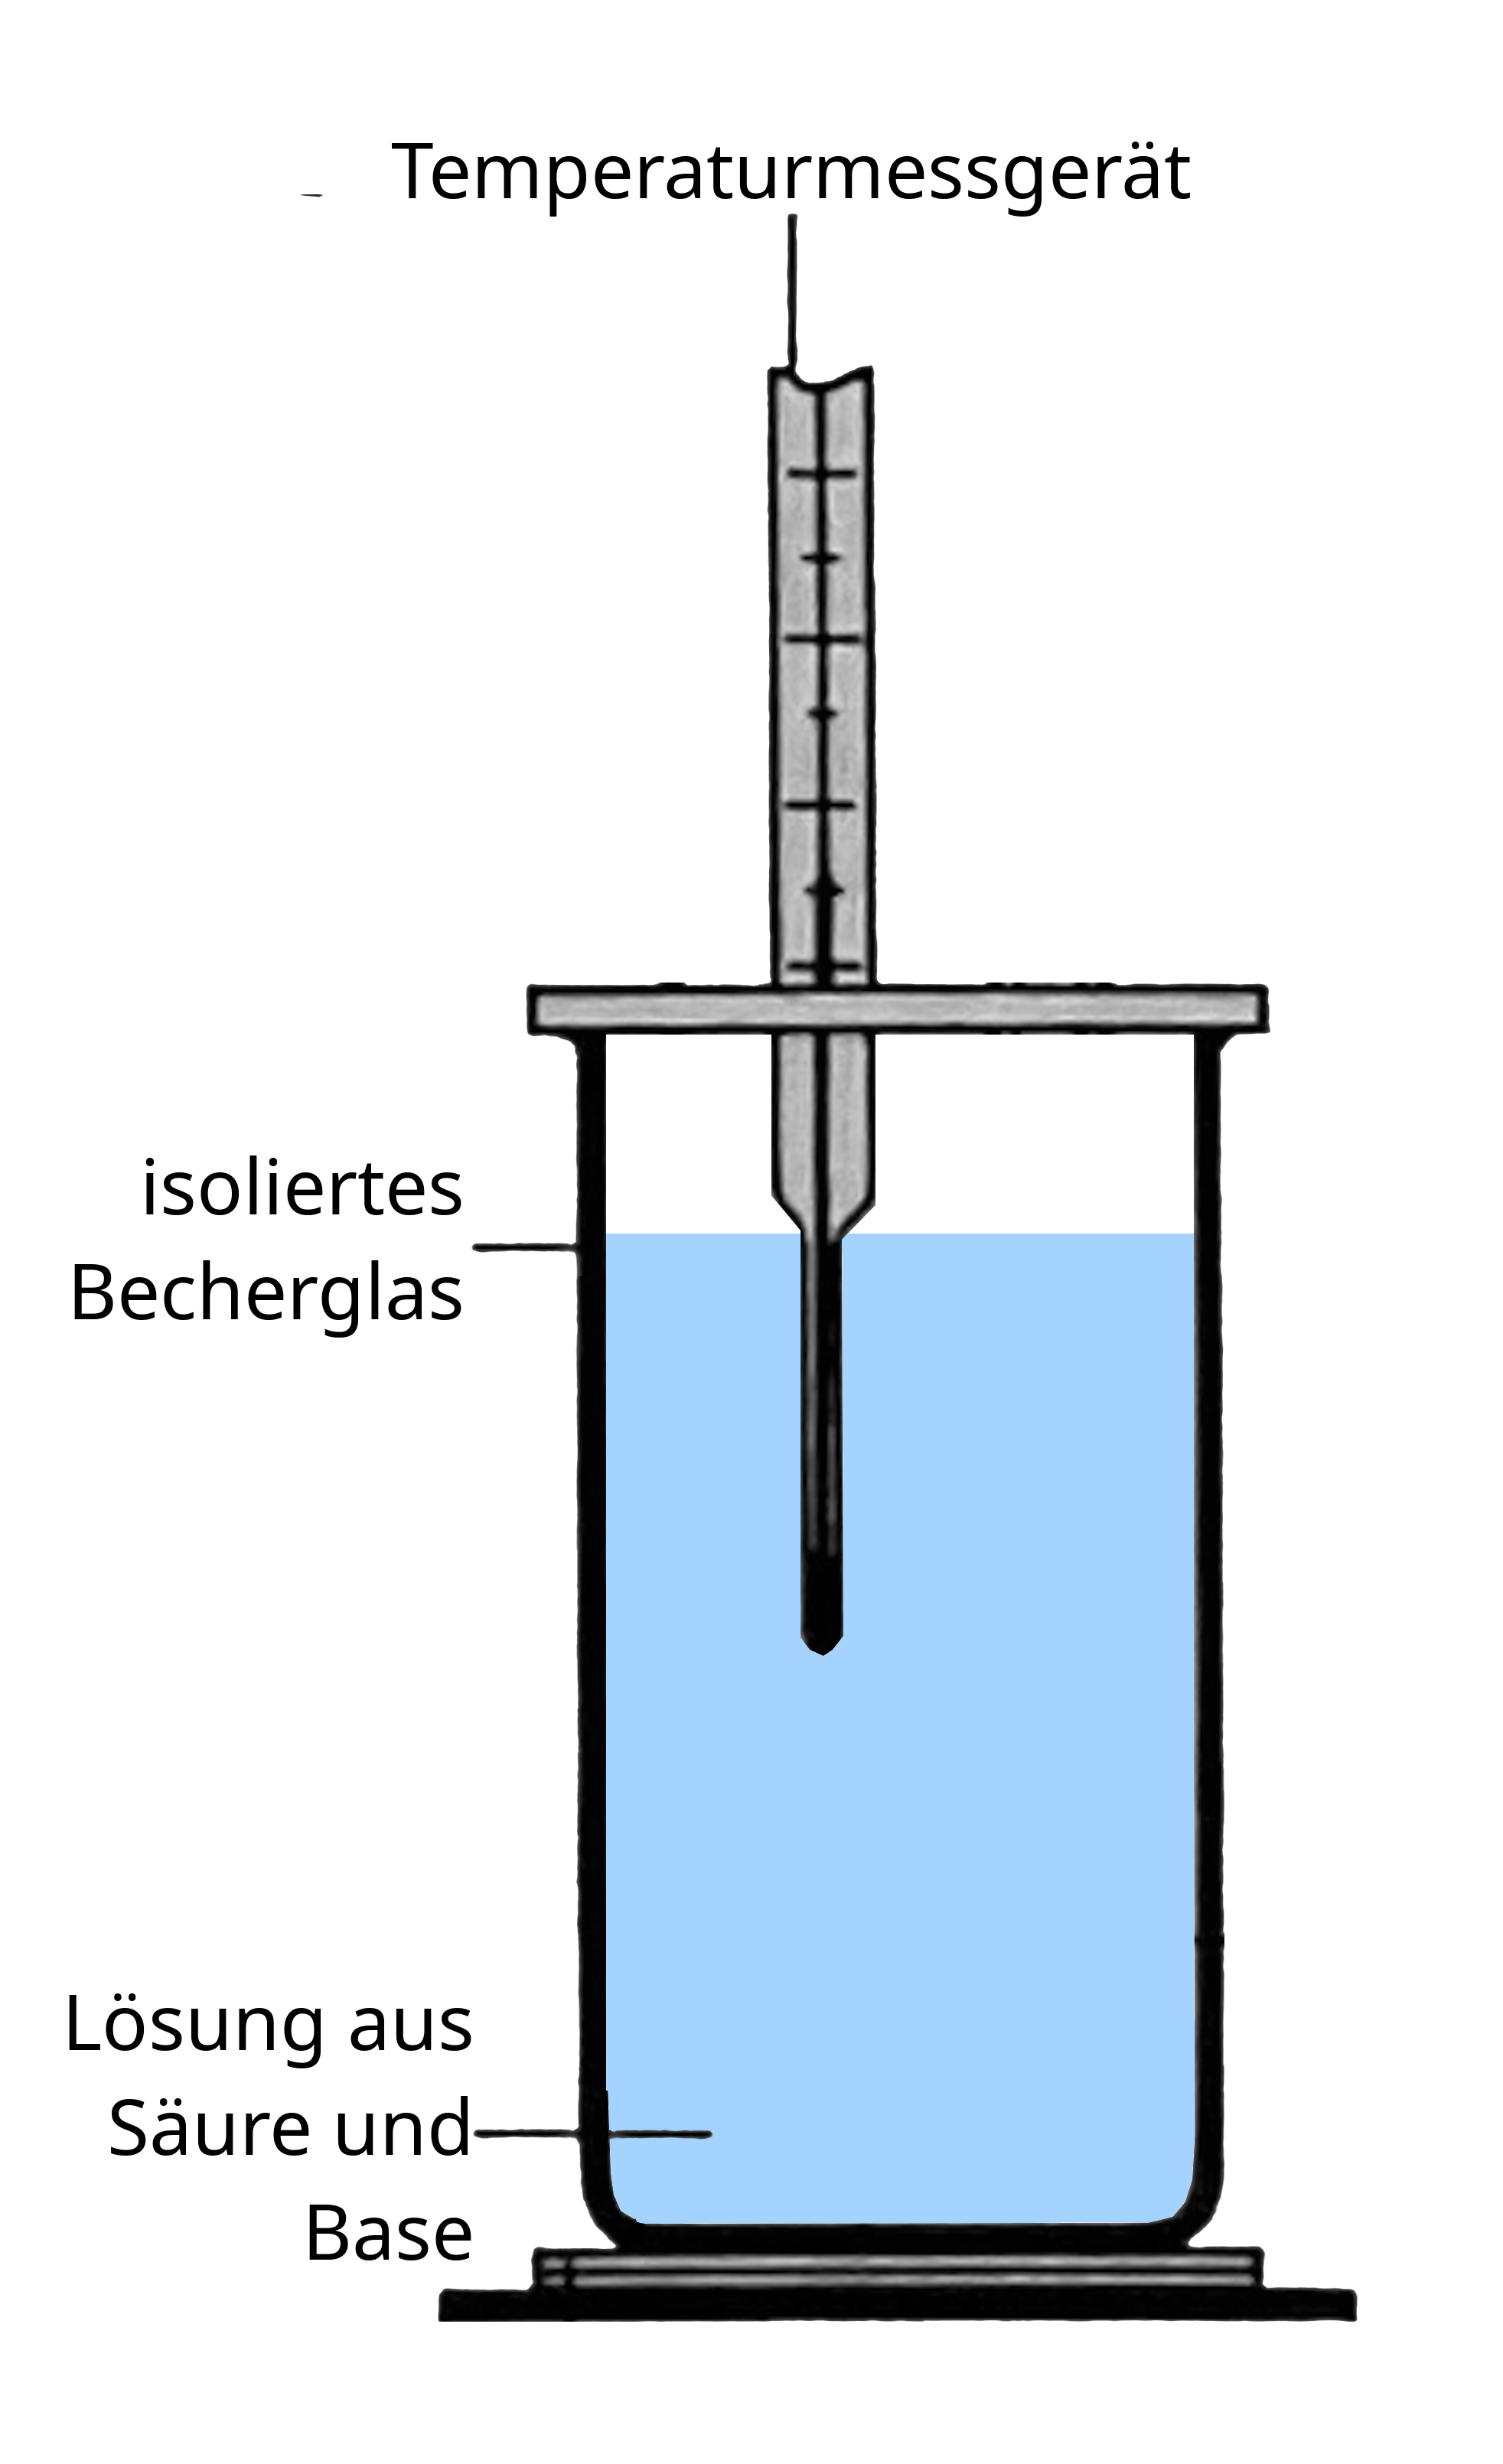
\includegraphics[width=0.33\textwidth]{Versuchsaufbau.png}
    \caption*{Ein beispielhafter Versuchsaufbau}
\end{figure*}

\subsection*{Durchführung}

\begin{enumerate}
    \item Lösungen von Säure und Base auf Raumtemperatur abkühlen lassen
    \item Temperaturmesser im isolierten Becherglas befestigen
    \item Säure und Base in das Becherglas füllen
    \item den Temperaturverlauf während der Neutralisationsreaktion messen
\end{enumerate}

\subsection*{Beobachtung}
\begin{tabular}{|c|c|}
    \hline
    Zeitpunkt $t$ in s & Temperatur $T$ in \textcelsius \\
    \hline
    0 & 21,5 \\
    10 & 21,6 \\
    20 & 21,7 \\
    30 & 21,7 \\
    40 & 21,7 \\
    50 & 21,8 \\
    52 & 21,8 \\
    54 & 22,7 \\
    56 & 23,5 \\
    58 & 24,1 \\
    60 & 24,6 \\
    62 & 24,9 \\
    64 & 25,2 \\
    66 & 25,3 \\
    68 & 25,5 \\
    70 & 25,6 \\
    80 & 25,8 \\
    90 & 25,8 \\
    100 = $T_\textrm{max}$ & 25,9 \\
    110 & 25,9 \\
    120 & 25,9 \\
    300 & 25,8 \\
    600 & 25,6 \\
    900 & 25,4 \\
    1200 & 25,3 \\
    \hline
\end{tabular}

\begin{tikzpicture}
\begin{axis}[
    axis lines=left,
    xlabel={Zeit in s},
    ylabel={Temperatur in \textcelsius},
    xmin=0, xmax=1200,
    ymin=0, ymax=30,
    xtick={0, 120, 240, 360, 480, 600, 720, 840, 960, 1080, 1200},
    ytick={0, 10, 20, 30, 40},
    legend pos=north west,
    ymajorgrids=true,
    grid style=dashed,
]

\addplot[
    color=blue,
    ]
    coordinates {
(0,21.533224105834961)(10,21.597570419311523)(20,21.672651290893555)(30,21.694097518920898)(40,21.72627067565918)(50,21.779897689819336)(60,24.557699203491211)(70,25.587308883666992)(80,25.791082382202148)(90,25.844709396362305)(100,25.887609481811523)(110,25.909063339233398)(120,25.930509567260742)(130,25.951963424682617)(140,25.951963424682617)(150,25.951963424682617)(160,25.94123649597168)(170,25.919790267944336)(180,25.909063339233398)(190,25.887609481811523)(200,25.86616325378418)(210,25.86616325378418)(220,25.855436325073242)(230,25.823263168334961)(240,25.823263168334961)(250,25.812536239624023)(260,25.823263168334961)(270,25.801809310913086)(280,25.791082382202148)(290,25.801809310913086)(300,25.780363082885742)(310,25.737462997436523)(320,25.758909225463867)(330,25.737462997436523)(340,25.726736068725586)(350,25.74818229675293)(360,25.716009140014648)(370,25.737462997436523)(380,25.705282211303711)(390,25.716009140014648)(400,25.683835983276367)(410,25.683835983276367)(420,25.683835983276367)(430,25.683835983276367)(440,25.67310905456543)(450,25.662382125854492)(460,25.651662826538086)(470,25.662382125854492)(480,25.651662826538086)(490,25.651662826538086)(500,25.651662826538086)(510,25.651662826538086)(520,25.640935897827148)(530,25.640935897827148)(540,25.630208969116211)(550,25.640935897827148)(560,25.630208969116211)(570,25.630208969116211)(580,25.619482040405273)(590,25.619482040405273)(600,25.630208969116211)(610,25.587308883666992)(620,25.587308883666992)(630,25.59803581237793)(640,25.587308883666992)(650,25.608762741088867)(660,25.565862655639648)(670,25.576581954956055)(680,25.576581954956055)(690,25.565862655639648)(700,25.544408798217773)(710,25.544408798217773)(720,25.565862655639648)(730,25.555135726928711)(740,25.533681869506836)(750,25.533681869506836)(760,25.533681869506836)(770,25.522954940795898)(780,25.522954940795898)(790,25.522954940795898)(800,25.512235641479492)(810,25.512235641479492)(820,25.501508712768555)(830,25.490781784057617)(840,25.490781784057617)(850,25.48005485534668)(860,25.469335556030273)(870,25.48005485534668)(880,25.469335556030273)(890,25.447881698608398)(900,25.447881698608398)(910,25.447881698608398)(920,25.447881698608398)(930,25.426435470581055)(940,25.426435470581055)(950,25.437154769897461)(960,25.40498161315918)(970,25.415708541870117)(980,25.40498161315918)(990,25.40498161315918)(1000,25.40498161315918)(1010,25.394254684448242)(1020,25.372808456420898)(1030,25.383535385131836)(1040,25.362081527709961)(1050,25.383535385131836)(1060,25.362081527709961)(1070,25.362081527709961)(1080,25.351354598999023)(1090,25.362081527709961)(1100,25.340635299682617)(1110,25.319181442260742)(1120,25.319181442260742)(1130,25.340635299682617)(1140,25.287008285522461)(1150,25.319181442260742)(1160,25.276281356811523)(1170,25.276281356811523)(1180,25.276281356811523)(1190,25.265554428100586)(1200,25.276281356811523)
    };
\end{axis}
\end{tikzpicture}

\subsection*{Auswertung}
\subsubsection*{Reaktionsgleichung}
$$ \ce{H2SO4 + 2NaOH} \rightarrow \ce{2H2O + 2Na+ + SO4^2-} $$

\subsubsection*{Berechnung}
Es wird die Temperaturdifferenz zwischen dem Ausgangszustand und dem Zeitpunkt der höchsten Temperatur während der Reaktion betrachtet:
\begin{align*}
    \Delta T &= T_\textrm{max} - T_0 \\
    &= 25,9 ^\circ\textrm{C} - 21,5 ^\circ\textrm{C}\\
    &= 4,4 \textrm{ K}
\end{align*}

Mithilfe dieser lässt sich die Neutralisationsenthalpie $\Delta_R H$ berechnen:

$$ \Delta_R H = - \frac{\Delta T \cdot c_p(\ce{H2O}) \cdot m(\ce{H2O})}{n_F} $$

Die Masse des Wassers ergibt sich aus dem Produkt aus den Dichten und den Volumina der Lösungen. Die Dichten lassen sich hierbei als die von Wasser annehmen, da es sich um wässrige Lösungen handelt:

\begin{align*}
    m(\ce{H2O}) &= \varrho(\ce{H2O}) \cdot (V(\ce{H2SO4}) + V(\ce{NaOH})) \\
    &= 1 \frac{\textrm{kg}}{\textrm l} \cdot (0,02 \textrm{ l} + 0,02 \textrm{ l}) \\
    &= 0,04 \textrm{ kg}
\end{align*}

Die funktionale Stöchiometriezahl $n_F$ entspricht der Stoffmenge an Wasser, die bei der Reaktion gebildet wird. Diese ist gleich der Stoffmenge an Hydroxid-Ionen, die in der Base vorhanden sind. Demnach gilt:

\begin{align*}
    n_F &= n(\ce{OH-}) \\
    &= n(\ce{NaOH}) \\
    &= V(\ce{NaOH}) \cdot c(\ce{NaOH}) \\
    &= 20 \textrm{ ml} \cdot 1 \frac{\textrm{mol}}{\textrm l}\\
    &= 0,02 \textrm{ mol}
\end{align*}

Nun können alle Werte in die Formel für die Neutralisationsenthalpie eingesetzt und der Wert berechnet werden:

\begin{align*}
    \Delta_R H &= - \frac{4,4 \textrm{ K} \cdot 4,19 \frac{\textrm{kJ}}{\textrm{kg} \cdot \textrm{K}} \cdot 0,04 \textrm{ kg}}{0,02 \textrm{ mol}} \\
    &\approx -36,9 \frac{\textrm{kJ}}{\textrm{mol}}
\end{align*}

\subsection*{Fehlerbetrachtung}
Der errechnete Wert für die Neutralisationsenthalpie kann aus verschiedenen Gründen vom reellen Wert abweichen. Zum Beispiel entsteht eine gewisse Ungenauigkeit bereits durch Messunsicherheiten. Außerdem ist das Becherglas nicht perfekt isoliert, was einen gewissen Messfehler erzeugt. Zudem wurde für die Säure- und Baselösung die spezifische Wärmekapazität und Dichte von Wasser angenommen – durch die gelösten Stoffe weicht der reelle Wert beider Größen allerdings ein wenig von denen von Wasser ab.

\end{document}